\chapter{Introduction} % Main chapter title
\label{chap:Chapter1}  % For referencing this chapter elsewhere, use \ref{Chapter1}
\epigraph{``Alone we can do so little, together we can do so much” }{\textit{Hellen Keller}}

Τα τελευταία χρόνια η ανάπτυξη της επιστήμης έχει επιφέρει την απόκτηση των 
τεχνολογικών επιτευγμάτων από το ευρύ κοινό με ένα πολύ οικονομικό αντίτιμο. Αυτό σημαίνει
ότι ο καθένας πολύ εύκολα μπορεί να έχει στην κατοχή του ακόμα και προϊόντα τα οποία θεωρούνται 
state-of-the-art χωρίς να χρειάζεται να δαπανήσει μεγάλα ποσά. 
Το ίδιο φυσικά, συμβαίνει και με τον κλάδο των drone και την - κατά επέκταση - χρήση αυτών $\cdot$ ακόμα και 
για ψυχαγωγικό σκοπό.  
\par
Κατά το τέλος του έτους 2019 μόνο στις Ηνωμένες Πολιτείες της Αμερικής υπήρχαν πάνω από 
990 χιλιάδες εγγεγραμμένοι χειριστές drone με πάνω από 1.32 εκατομμύρια drone ψυχαγωγικού 
χαρακτήρα να χρησιμοποιούνται \cite{2019-drone-statistic}. Ενώ μέχρι το 2025 υπολογίζεται 
ότι το μέγεθος αγοράς των υπηρεσιών drone θα κοστολογείται στα 63.6 εκατομμύρια δολάρια \cite{expected-drone-market}.
\par
Φυσικά η χρήση τους δεν περιορίζεται μόνο στην ψυχαγωγία, εταιρίες όπως η Amazon έχουν 
αποκτήσει ήδη τα απαραίτητα πιστοποιητικά και εγκρίσεις και σκοπεύουν να 
χρησιμοποιήσουν drone για παράδοση των δεμάτων \cite{amazon-drones} αρκετά σύντομα, καθώς προς το παρόν
η διαδικασία βρίσκεται σε στάδιο δοκιμών. 
Συνεπώς είναι εύκολο να κατανοηθεί ότι ο συγκεκριμένος κλάδος πρόκειται να έχει ακόμα μεγαλύτερη 
άνθιση, με αρκετά μεγάλο ερευνητικό ενδιαφέρον να του αναλογεί.   
\par
Με την αύξηση των drone και την αύξηση των εφαρμογών, υπάρχει η ανάγκη συνεργασίας και η δημιουργία drone swarms 
για την επιτυχή ολοκλήρωση των στόχων που έχουν οριστεί. Όμως για να καταφέρουν τα drone
να συνεργαστούν χρειάζεται πρώτα να μπορούν να ξεπεράσουν τα προβλήματα τα οποία υπάρχουν.

\newpage

%----------------------------------------------------------------------------------------
%	SECTION 1
%----------------------------------------------------------------------------------------
\section{UAV and Swarm} \label{sec:Chapter1-1} 

Είναι σημαντικό από τα πρώτα βήματα, να έχει γίνει κατανοητό με τον όρο drone σε τι 
παραπέμπουμε - όπως επίσης πότε θεωρείται ότι ένα σμήνος από drone πετάει σε σχηματισμό (drone swarm).

%----------------------------------------------------------------------------------------
\subsection{UAV}    \label{sec:Chapter1-1-1}
Όταν αναφερόμαστε στον όρο Unmanned aerial vehicle (\hyperref[abbr:UAV]{UAV}) ή απλούστερα drone 
κάνουμε αναφορά για ένα μη επανδρωμένο ιπτάμενο αεροσκάφος το οποίο ελέγχεται είτε απομακρυσμένα από
έναν άνθρωπο, είτε είναι τελείως αυτόνομο. Τα \hyperref[abbr:UAV]{UAV} μαζί με ένα σταθμό βάσης και την
από κοινού επικοινωνίας του σταθμού - drone, δημιουργούν αυτό που ονομάζουμε Unmanned aircraft 
system (\hyperref[abbr:UAS]{UAS}) \cite{what-is-UAV} \cite{what-is-UAV-and-history}.

Η πρώτη εμφάνιση των \hyperref[abbr:UAV]{UAV} έγινε κατά το 1849 στα πλαίσια μάχης, ενώ οι πρώτες 
καινοτομίες πάνω σε αυτά ξεκίνησαν ήδη από τις αρχές του 20ου αιώνα. Το 2013 τουλάχιστον 50 χώρες 
χρησιμοποιούσαν \hyperref[abbr:UAV]{UAVs} για κάποιον σκοπό, με μερικές από αυτές φυσικά να 
σχεδιάζουν τα δικά τους \cite{what-is-UAV-and-history}.
Αυτήν την στιγμή υπάρχουν πάνω από 1000 διαφορετικά μοντέλα \hyperref[abbr:UAV]{UAV} που χρησιμοποιούνται
ανά τον κόσμο, με τα περισσότερα από αυτά να μην έχουν ψυχαγωγικό χαρακτήρα
\cite{list-of-UAVs}. 
\par
Είναι λοιπόν ξεκάθαρο ότι το πλήθος των drone είναι τόσο μεγάλο, λόγω των διαφορετικών αναγκών - και ότι κάποια έχουν καλύτερα
αποτελέσματα από ότι άλλα σε συγκεκριμένες αποστολές. Για αυτό, έχουν γίνει 
ήδη προσπάθειες για την κατηγοριοποίηση των \hyperref[abbr:UAV]{UAVs} σύμφωνα με τα διάφορα χαρακτηριστικά που μπορεί να έχουν.
Ενδεικτικά με βάση το μέγεθος, την αυτονομία, το βάρος ή το μηχανολογικό σχεδιασμό των \hyperref[abbr:UAV]{UAV}
είναι μερικές από τις υπάρχουσες \cite{what-is-UAV}
\cite{drone-classification} \cite{application-areas|swarm-types|uavs-classification|sensor's-used|swarms-problems|public-awareness}.
Στο Table \ref{tab:drone-determined-by-their-structure} υπάρχει μία απλουστευμένη κατηγοριοποίηση η οποία προτάθηκε
από τους συγγραφείς του \cite{application-areas|swarm-types|uavs-classification|sensor's-used|swarms-problems|public-awareness}
σύμφωνα με τη βασική μηχανολογική δομή που μπορεί να έχει ένα drone καθώς και τα πλεονεκτήματα της κάθε δομής. 

\begin{table}[H]
    \caption{Κατηγοριοποίηση των UAV βάση της δομή τους \cite{application-areas|swarm-types|uavs-classification|sensor's-used|swarms-problems|public-awareness}.}
    \label{tab:drone-determined-by-their-structure}
    \centering
    \begin{tabular}{llll}
        \toprule
        \textbf{Drones} & \textbf{Main features}  \\
        \midrule
            Fixed-Wing & long endurance and fast flight speed \\
            Fixed-Wing Hybrid & \hyperref[abbr:VTOL]{VTOL} and long endurance flight \\
            Single Rotor & \hyperref[abbr:VTOL]{VTOL}, hover, and long endurance flight \\
            Multirotor & \hyperref[abbr:VTOL]{VTOL}, hover, and short endurance flight \\
        \bottomrule
    \end{tabular}
\end{table}

\begin{figure} [H]
    \centering
    % -----------------
    \begin{minipage}{.5\textwidth}
      \centering
      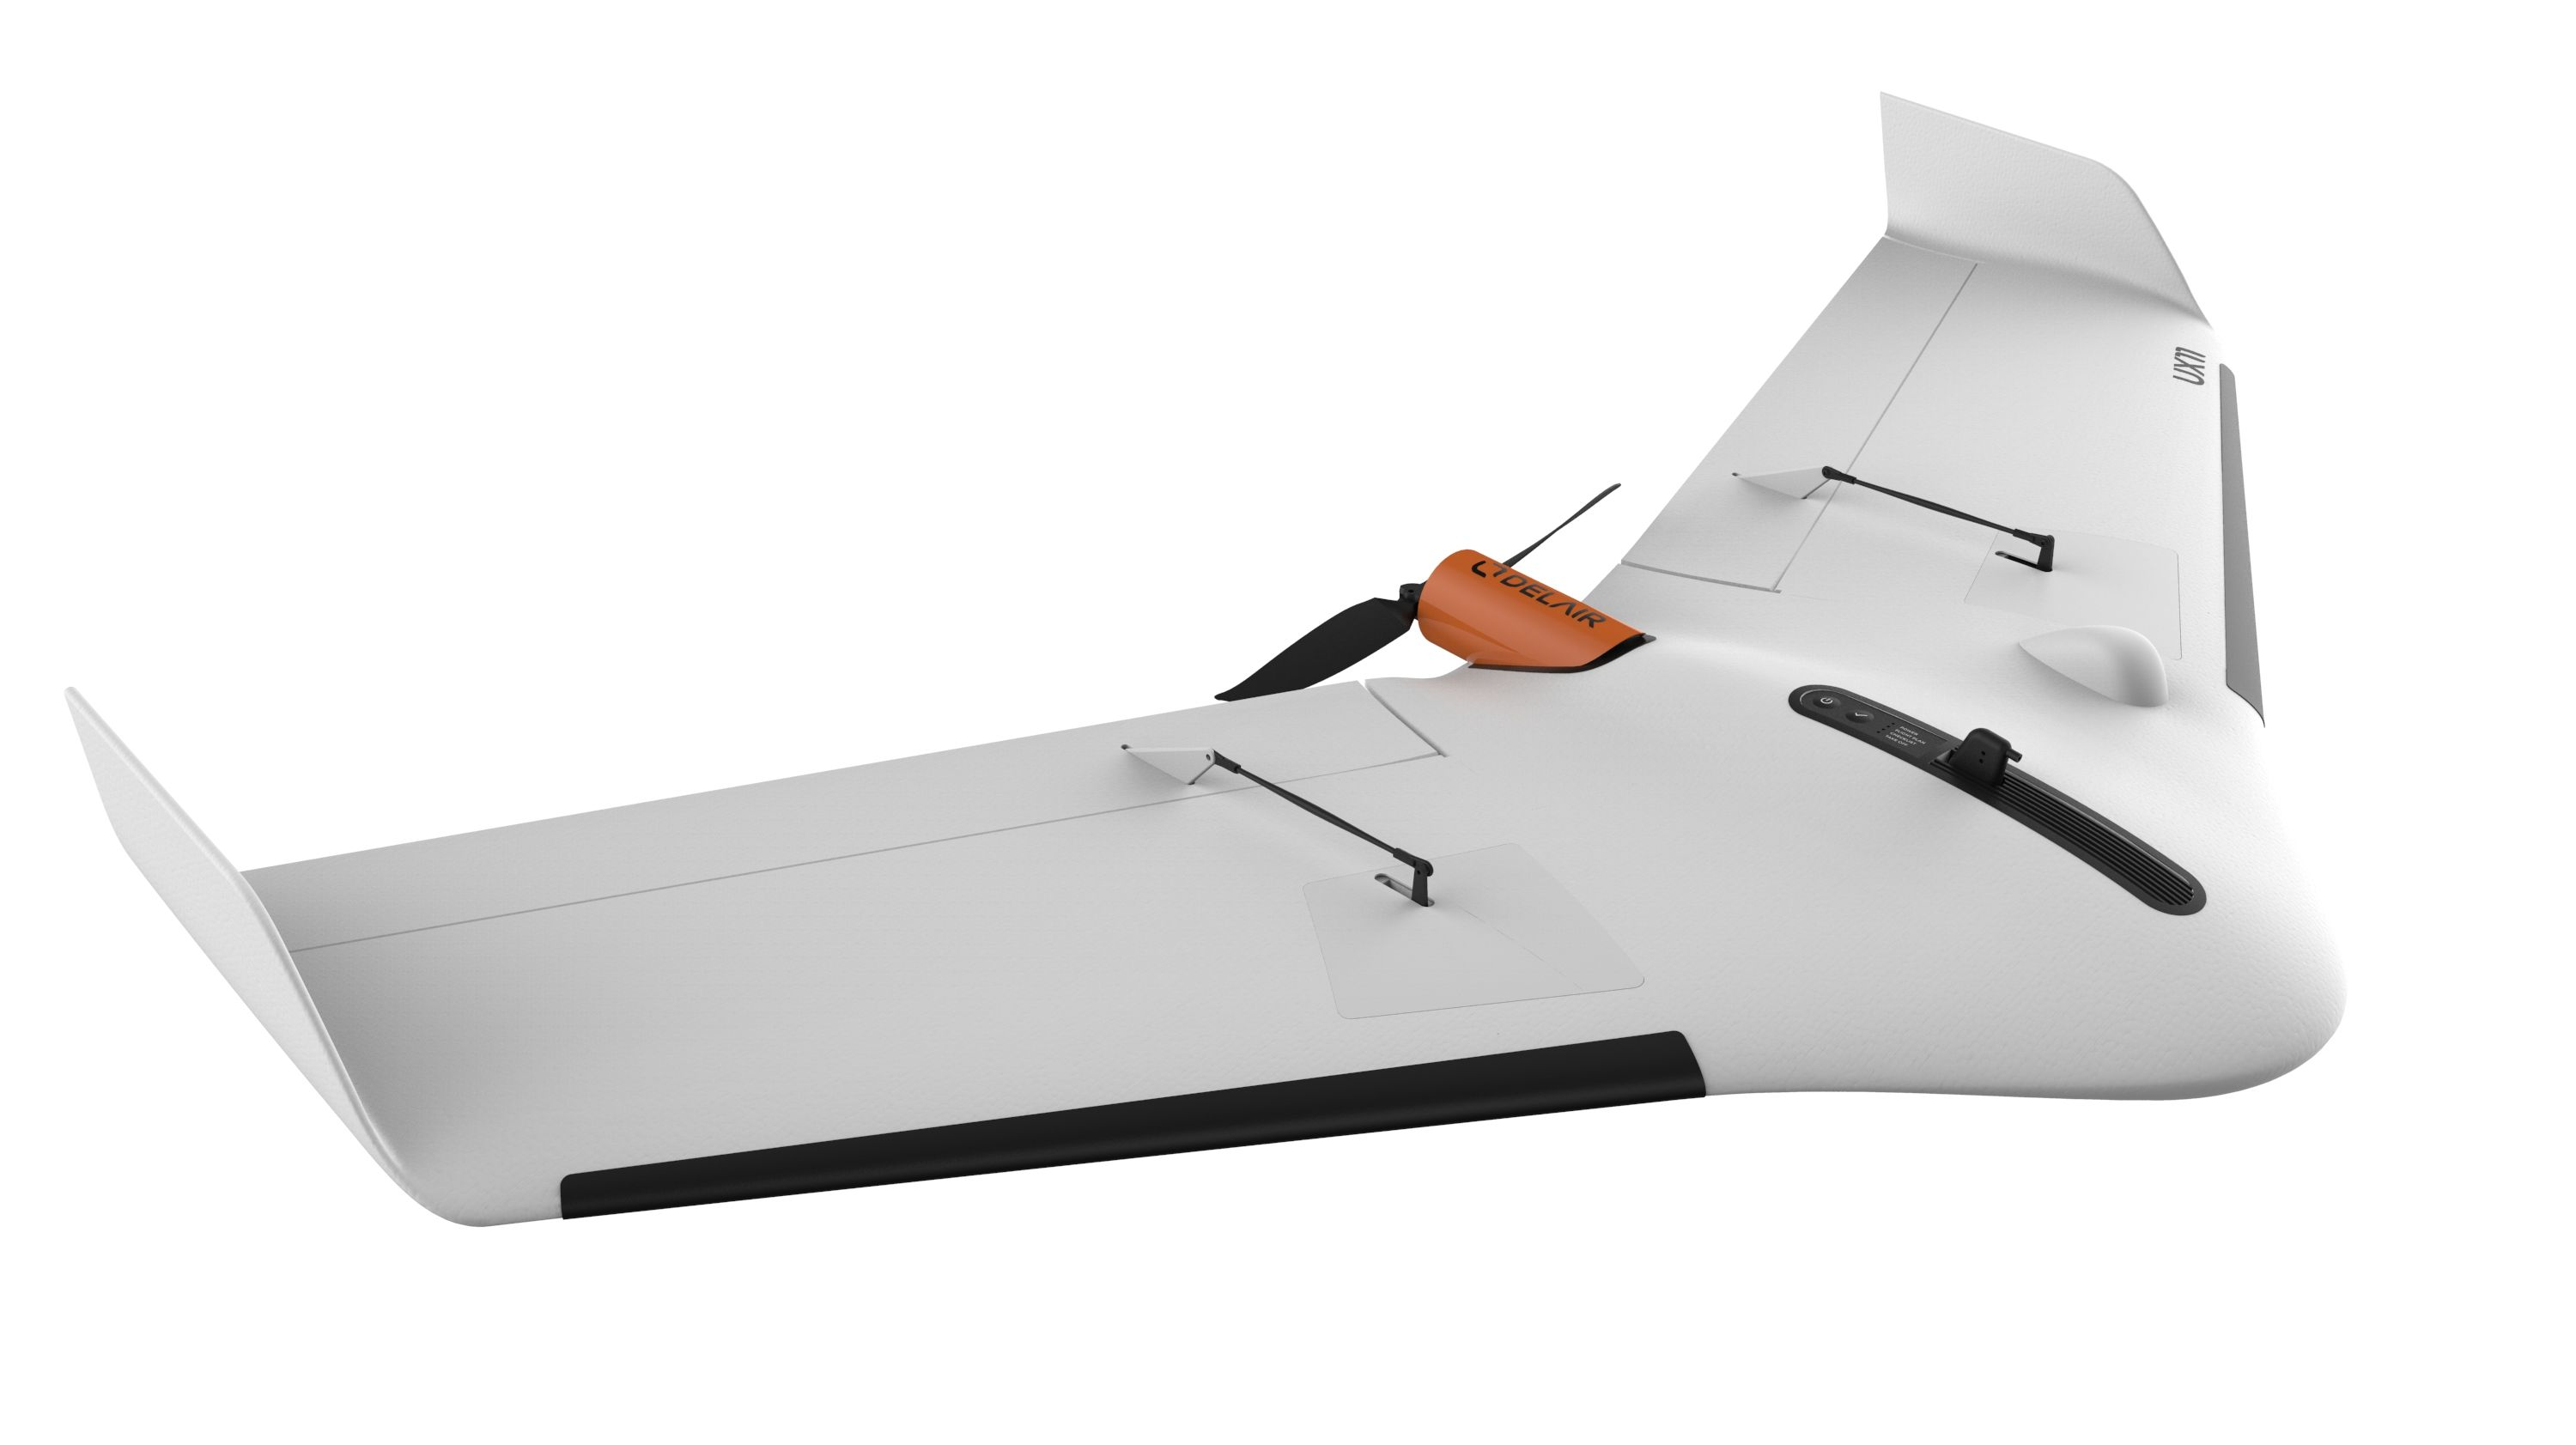
\includegraphics[width=\linewidth]{Images/Introduction/uav-fixed-wing-example.jpg}
      {(a) Fixed-Wing} (\href{https://delair.aero/portfolio/surveying-and-mapping/}{URL})
    \end{minipage}%
    % -----------------
    \begin{minipage}{.5\textwidth}
      \centering
      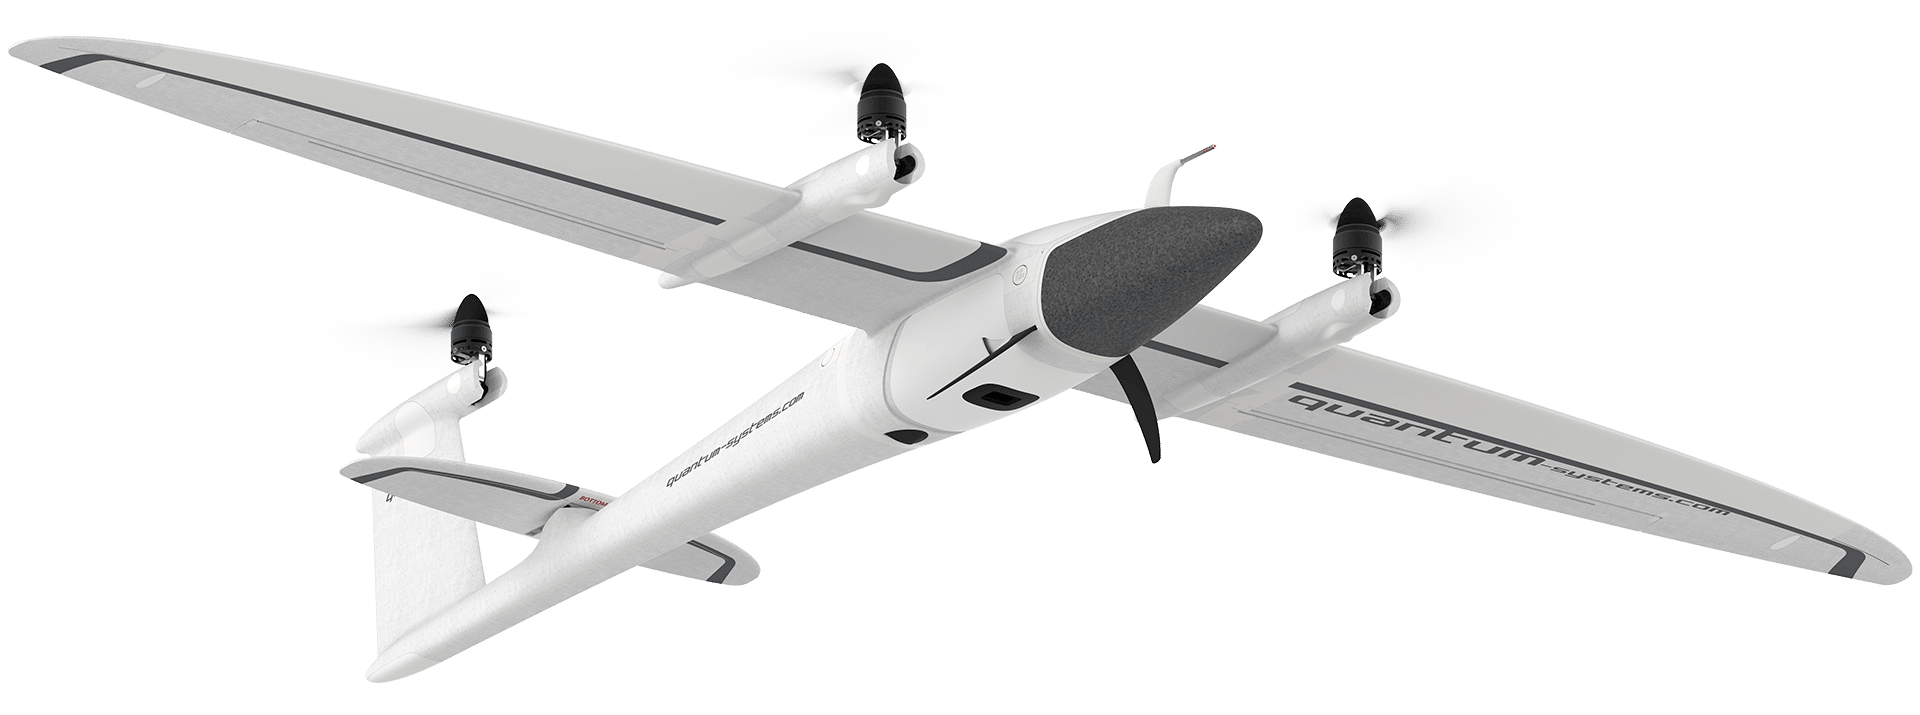
\includegraphics[width=\linewidth]{Images/Introduction/uav-fixed-wing-hybrid-example.png}
      {(b) Fixed-Wing Hybrid} (\href{https://www.quantum-systems.com/project/trinity-f90/}{URL})
    \end{minipage}
    % -----------------
    \begin{minipage}{.5\textwidth}
        \centering
        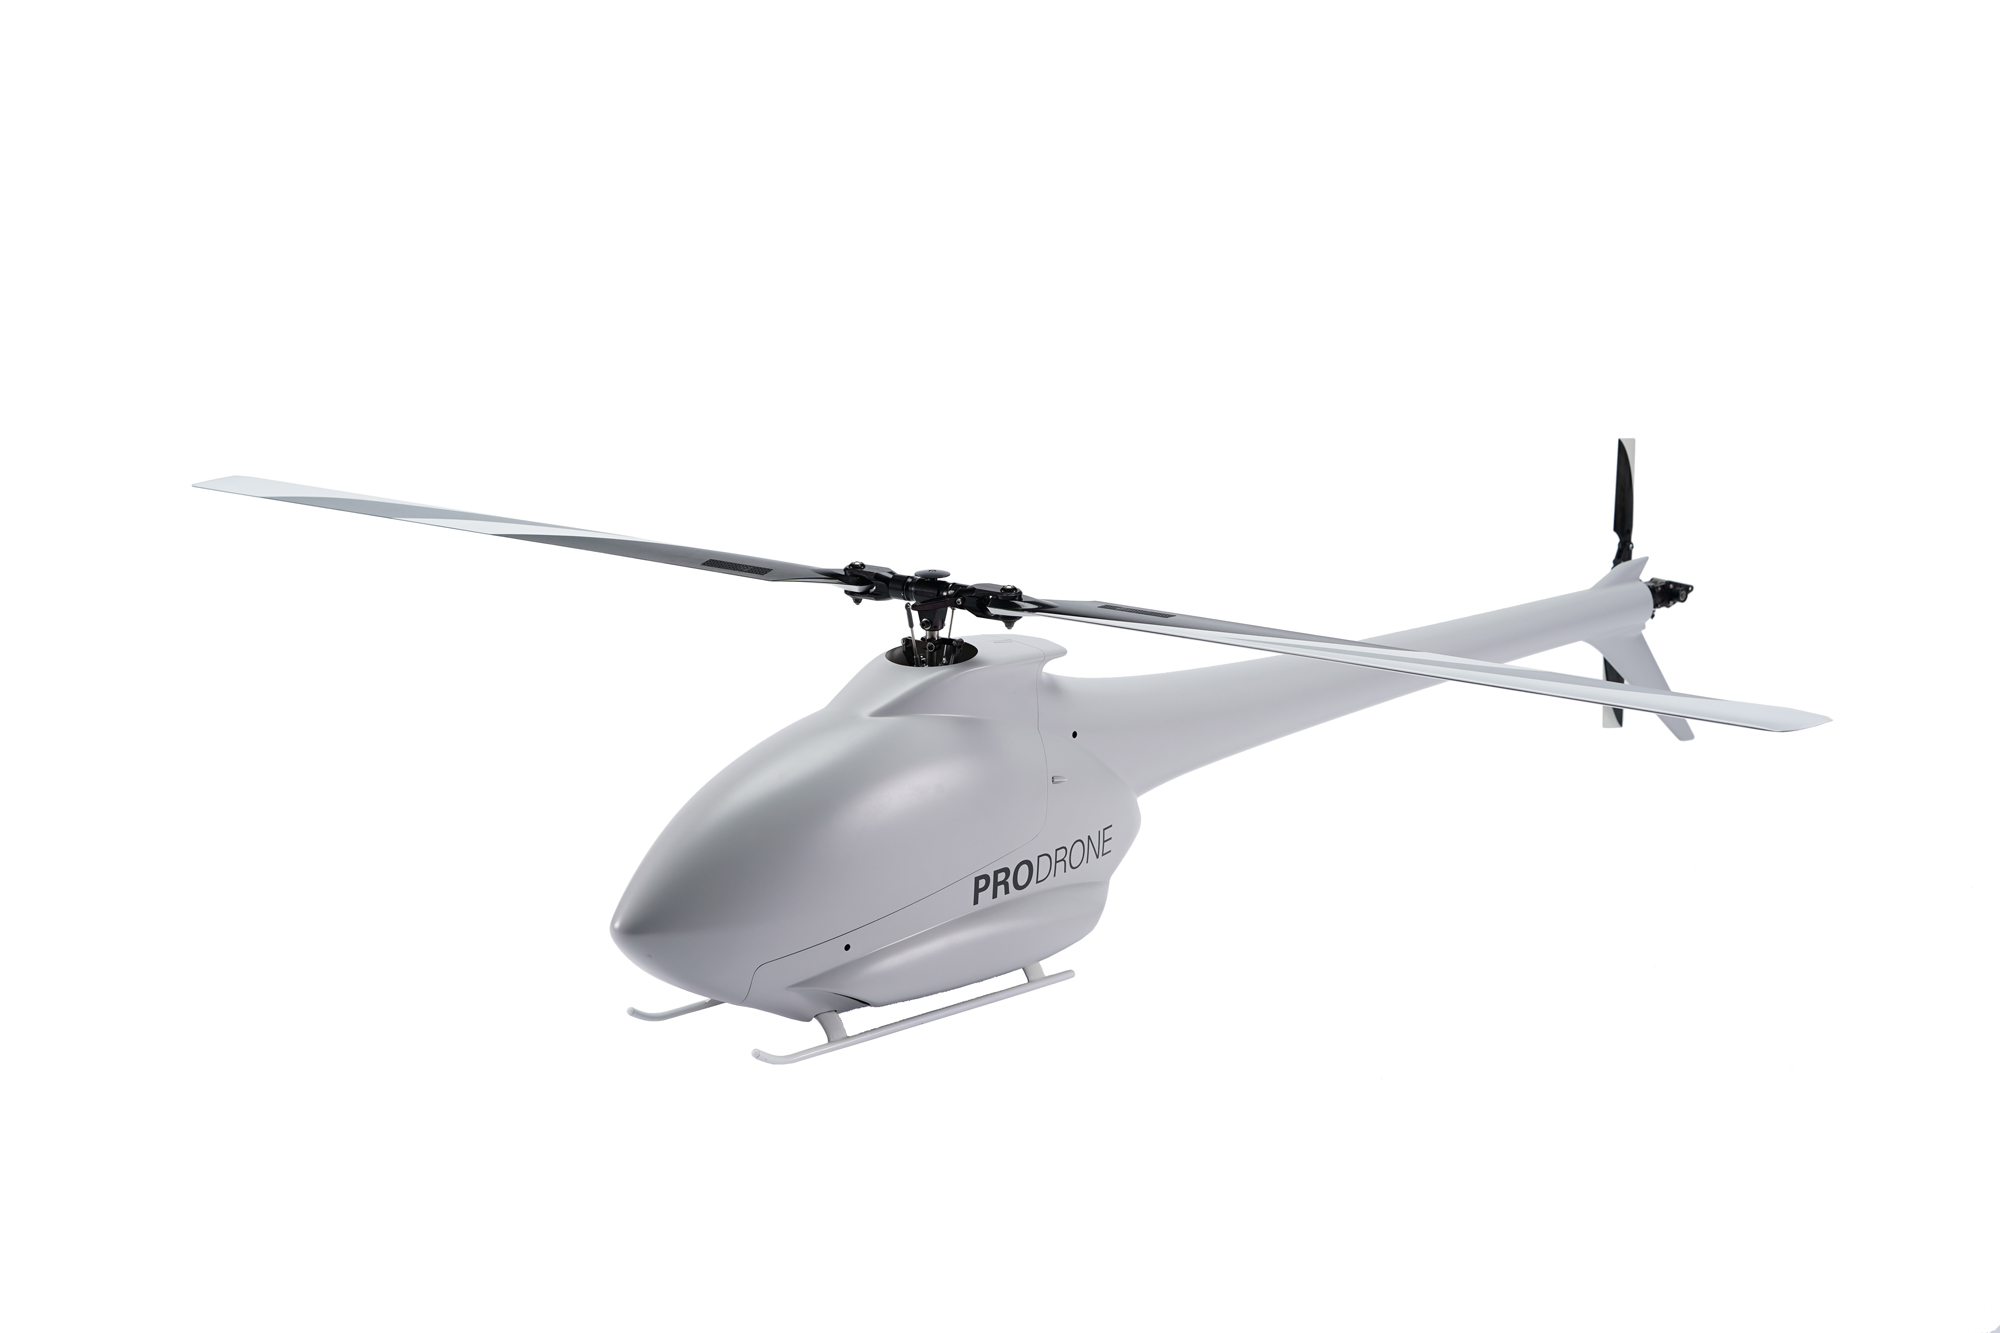
\includegraphics[width=\linewidth]{Images/Introduction/uav-single-rotor-example.jpg}
        {(c) Single Rotor} (\href{https://www.prodrone.com/release-en/2874/}{URL})
      \end{minipage}%
      % -----------------
      \begin{minipage}{.5\textwidth}
        \centering
        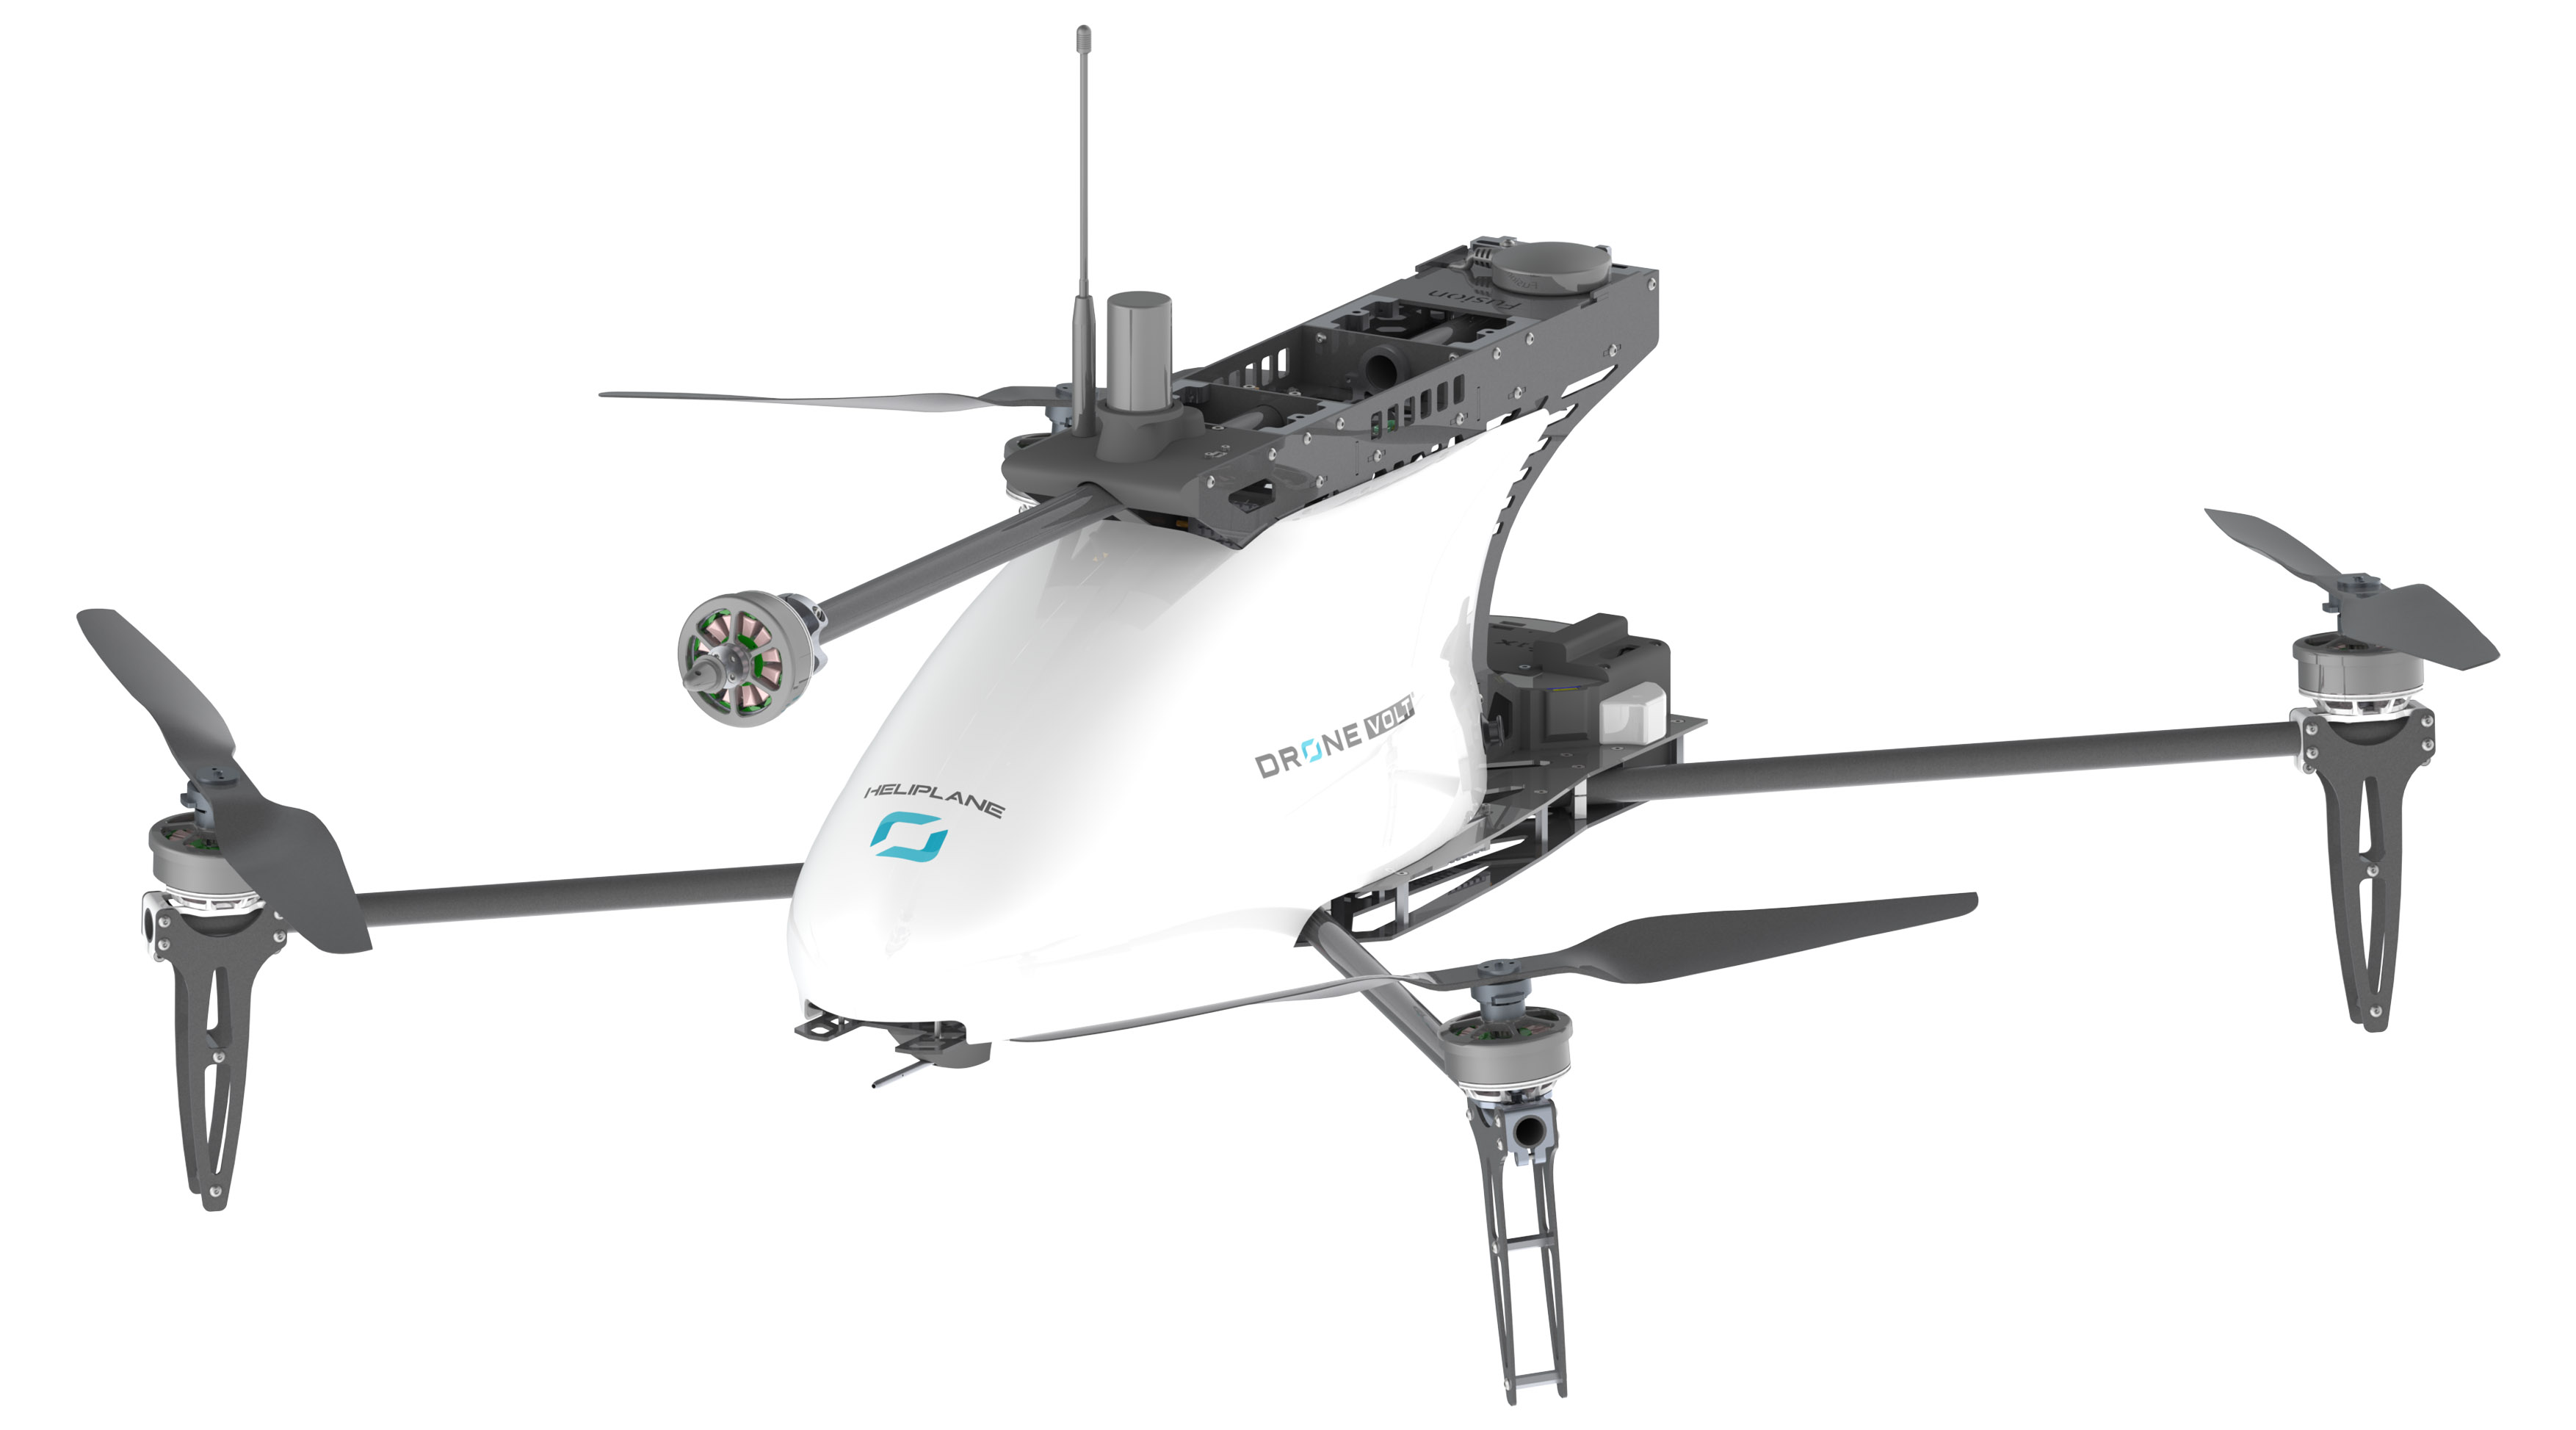
\includegraphics[width=\linewidth]{Images/Introduction/uav-multirotor-example.jpg}
        {(d) Multirotor} (\href{https://metatronus.com/heliplane/}{URL})
      \end{minipage}
      % -----------------
    \hfill \break
    \decoRule
    \caption[UAV Examples]{}
    \label{fig:UAV-samples}
\end{figure}

Τυπικά τα Fixed-Wing drones είναι αρκετά ακριβά, χρειάζονται εξειδικευμένους χει- ριστές για να
λειτουργήσουν, όπως επιπλέον και περισσότερο χώρο για την απογείωση και την προσγείωση. Είναι 
ιδανικά για εφαρμογές που χρειάζεται να καλύψουμε μεγάλες περιοχές και συχνά έχουν αυτονομία 
τουλάχιστον μερικών ωρών. Για αυτούς τους λόγους χρησιμοποιούνται κυρίως από κυβερνήσεις,
στρατιωτικές μονάδες ή επιχειρήσεις για την γρήγορη επίβλεψη μεγάλων εκτάσεων \cite{fixed-wing}.  

Τα Fixed-Wing Hybrid προσπαθούν να λύσουν τα μειονεκτήματα που έχουν τα Fixed-Wing drones, την μη ικανότητα 
δηλαδή για  Vertically Hover, Take-off, and Land (\hyperref[abbr:VTOL]{VTOL}) όμως είναι ακόμα σε αρχικά στάδια.

Τα Single Rotor είναι επίσης αρκετά ακριβά, πολύπλοκα μηχανολογικά μηχανήμα- τα, που δέχονται πολλούς κραδασμούς, 
απαιτούν εξειδικευμένους χειριστές όμως μπορούν να μεταφέρουν αρκετά βαριά payloads, θετικό στην χρήση τους ότι 
μπορούν να πραγματοποιήσουν \hyperref[abbr:VTOL]{VTOL}.

Τα Multirotor είναι ίσως τα πιο ευρέως διαδεδομένα. Καθώς είναι τα πιο οικονομικά από τα παραπάνω και εύκολο να κατασκευαστούν.
Μπορούν να βρεθούν στο εμπόριο με διάφορο πλήθος από έλικες και είναι το κύριο είδος που χρησιμοποιείται από ερασιτέχνες
ή χομπίστες για λόγους αναψυχής.

Στο Figure \ref{fig:UAV-samples} δίνονται κάποια ενδεικτικά παραδείγματα \hyperref[abbr:UAV]{UAVs} με βάση την κατηγοριοποίηση
του Table \ref{tab:drone-determined-by-their-structure}.
Φυσικά αυτή η κατηγοριοποίηση δεν περιλαμβάνει όλα τα είδη drone, είναι όμως ικανοποιητική για να γίνουν
ξεκάθαρα δύο βασικές ιδέες. Αρχικά ανάλογα με την εφαρμογή που μας ενδιαφέρει, θα πρέπει να επιλέξουμε
την χρήση του πλέον κατάλληλου τύπου drone. Όπως επίσης με βάση την επιλογή του συγκεκριμένου τύπου -
αυτόματα έχουμε να διαχειριστούμε τα πλεονεκτήματα ή τα μειονεκτήματα που έχει.

Σε περίπτωση που μας ενδιαφέρει, οι συγγραφείς του \cite{drone-classification} παρουσιάζουν 
με εκτενέστερο τρόπο διάφορες κατηγοριοποιήσεις
και είδη drone τα οποία δεν εμπίπτουν στα πλαίσια αυτής της διπλωματικής και κυμαίνονται 
από smart dust, bio-drones, hybrid drones και άλλα πολλά.

Σε όποια από τις κατηγορίες και αν αντιστοιχεί ένα \hyperref[abbr:UAV]{UAV}
από την στιγμή που είναι ένα ιπτάμενο αντικείμενο, θα πρέπει να έχει την δυνατότητα να κινείται -
φυσικά - στον αέρα. Στο Figure \ref{fig:UAV-principal-axes} παρουσιάζονται στους 3 άξονες οι κινήσεις
ενός \hyperref[abbr:UAV]{UAV} \cite{aircraft-principal-axes}.

\begin{figure} [H]
	\centering
	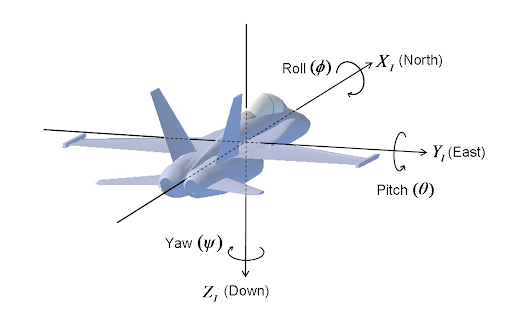
\includegraphics[scale=0.6]{Images/Introduction/aircraft-principal-axes.png}
	\decoRule
	\caption[UAV]{\hyperref[abbr:UAV]{UAV} principal axes: \href{http://www.chrobotics.com/library/understanding-euler-angles}{URL}}
	\label{fig:UAV-principal-axes}
\end{figure}

Κάτι ακόμα σημαντικό είναι το πλήθος και είδος των αισθητήρων που υπάρχουν πλέον πάνω στα drones.
Με τους 

%----------------------------------------------------------------------------------------
\subsection{Swarms} \label{sec:Chapter1-1-2}


%----------------------------------------------------------------------------------------
%	SECTION 2
%----------------------------------------------------------------------------------------
\section{Motivation} \label{sec:Chapter1-2} 

TODO: χρήση των drone

%----------------------------------------------------------------------------------------
%	SECTION 3
%----------------------------------------------------------------------------------------
\section{Scientific Goals and Contributions} \label{sec:Chapter1-3} 
TODO: Σκοπός αυτής της διπλωματικής

%----------------------------------------------------------------------------------------
%	SECTION 4
%----------------------------------------------------------------------------------------
\section{Thesis Outline} \label{sec:Chapter1-4} 

    \begin{itemize}
        \item \textbf{Chapter 2 - {\hypersetup{hidelinks}\nameref{chap:Chapter2}}:}
        \item \textbf{Chapter 3 - {\hypersetup{hidelinks}\nameref{chap:Chapter3}}:}
        \item \textbf{Chapter 4 - {\hypersetup{hidelinks}\nameref{chap:Chapter4}}:}                %Maybe rename chapter's name
        \item \textbf{Chapter 5 - {\hypersetup{hidelinks}\nameref{chap:Chapter5}}:}       %Maybe rename chapter's name
        \item \textbf{Chapter 6 - {\hypersetup{hidelinks}\nameref{chap:Chapter6}}:}
        \item \textbf{Chapter 7 - {\hypersetup{hidelinks}\nameref{chap:Chapter7}}:}
    \end{itemize}
